\documentclass[11pt]{article}

    \usepackage[breakable]{tcolorbox}
    \usepackage{parskip} % Stop auto-indenting (to mimic markdown behaviour)
    
    \usepackage{iftex}
    \ifPDFTeX
    	\usepackage[T1]{fontenc}
    	\usepackage{mathpazo}
    \else
    	\usepackage{fontspec}
    \fi

    % Basic figure setup, for now with no caption control since it's done
    % automatically by Pandoc (which extracts ![](path) syntax from Markdown).
    \usepackage{graphicx}
    % Maintain compatibility with old templates. Remove in nbconvert 6.0
    \let\Oldincludegraphics\includegraphics
    % Ensure that by default, figures have no caption (until we provide a
    % proper Figure object with a Caption API and a way to capture that
    % in the conversion process - todo).
    \usepackage{caption}
    \DeclareCaptionFormat{nocaption}{}
    \captionsetup{format=nocaption,aboveskip=0pt,belowskip=0pt}

    \usepackage[Export]{adjustbox} % Used to constrain images to a maximum size
    \adjustboxset{max size={0.9\linewidth}{0.9\paperheight}}
    \usepackage{float}
    \floatplacement{figure}{H} % forces figures to be placed at the correct location
    \usepackage{xcolor} % Allow colors to be defined
    \usepackage{enumerate} % Needed for markdown enumerations to work
    \usepackage{geometry} % Used to adjust the document margins
    \usepackage{amsmath} % Equations
    \usepackage{amssymb} % Equations
    \usepackage{textcomp} % defines textquotesingle
    % Hack from http://tex.stackexchange.com/a/47451/13684:
    \AtBeginDocument{%
        \def\PYZsq{\textquotesingle}% Upright quotes in Pygmentized code
    }
    \usepackage{upquote} % Upright quotes for verbatim code
    \usepackage{eurosym} % defines \euro
    \usepackage[mathletters]{ucs} % Extended unicode (utf-8) support
    \usepackage{fancyvrb} % verbatim replacement that allows latex
    \usepackage{grffile} % extends the file name processing of package graphics 
                         % to support a larger range
    \makeatletter % fix for grffile with XeLaTeX
    \def\Gread@@xetex#1{%
      \IfFileExists{"\Gin@base".bb}%
      {\Gread@eps{\Gin@base.bb}}%
      {\Gread@@xetex@aux#1}%
    }
    \makeatother

    % The hyperref package gives us a pdf with properly built
    % internal navigation ('pdf bookmarks' for the table of contents,
    % internal cross-reference links, web links for URLs, etc.)
    \usepackage{hyperref}
    % The default LaTeX title has an obnoxious amount of whitespace. By default,
    % titling removes some of it. It also provides customization options.
    \usepackage{titling}
    \usepackage{longtable} % longtable support required by pandoc >1.10
    \usepackage{booktabs}  % table support for pandoc > 1.12.2
    \usepackage[inline]{enumitem} % IRkernel/repr support (it uses the enumerate* environment)
    \usepackage[normalem]{ulem} % ulem is needed to support strikethroughs (\sout)
                                % normalem makes italics be italics, not underlines
    \usepackage{mathrsfs}
    

    
    % Colors for the hyperref package
    \definecolor{urlcolor}{rgb}{0,.145,.698}
    \definecolor{linkcolor}{rgb}{.71,0.21,0.01}
    \definecolor{citecolor}{rgb}{.12,.54,.11}

    % ANSI colors
    \definecolor{ansi-black}{HTML}{3E424D}
    \definecolor{ansi-black-intense}{HTML}{282C36}
    \definecolor{ansi-red}{HTML}{E75C58}
    \definecolor{ansi-red-intense}{HTML}{B22B31}
    \definecolor{ansi-green}{HTML}{00A250}
    \definecolor{ansi-green-intense}{HTML}{007427}
    \definecolor{ansi-yellow}{HTML}{DDB62B}
    \definecolor{ansi-yellow-intense}{HTML}{B27D12}
    \definecolor{ansi-blue}{HTML}{208FFB}
    \definecolor{ansi-blue-intense}{HTML}{0065CA}
    \definecolor{ansi-magenta}{HTML}{D160C4}
    \definecolor{ansi-magenta-intense}{HTML}{A03196}
    \definecolor{ansi-cyan}{HTML}{60C6C8}
    \definecolor{ansi-cyan-intense}{HTML}{258F8F}
    \definecolor{ansi-white}{HTML}{C5C1B4}
    \definecolor{ansi-white-intense}{HTML}{A1A6B2}
    \definecolor{ansi-default-inverse-fg}{HTML}{FFFFFF}
    \definecolor{ansi-default-inverse-bg}{HTML}{000000}

    % commands and environments needed by pandoc snippets
    % extracted from the output of `pandoc -s`
    \providecommand{\tightlist}{%
      \setlength{\itemsep}{0pt}\setlength{\parskip}{0pt}}
    \DefineVerbatimEnvironment{Highlighting}{Verbatim}{commandchars=\\\{\}}
    % Add ',fontsize=\small' for more characters per line
    \newenvironment{Shaded}{}{}
    \newcommand{\KeywordTok}[1]{\textcolor[rgb]{0.00,0.44,0.13}{\textbf{{#1}}}}
    \newcommand{\DataTypeTok}[1]{\textcolor[rgb]{0.56,0.13,0.00}{{#1}}}
    \newcommand{\DecValTok}[1]{\textcolor[rgb]{0.25,0.63,0.44}{{#1}}}
    \newcommand{\BaseNTok}[1]{\textcolor[rgb]{0.25,0.63,0.44}{{#1}}}
    \newcommand{\FloatTok}[1]{\textcolor[rgb]{0.25,0.63,0.44}{{#1}}}
    \newcommand{\CharTok}[1]{\textcolor[rgb]{0.25,0.44,0.63}{{#1}}}
    \newcommand{\StringTok}[1]{\textcolor[rgb]{0.25,0.44,0.63}{{#1}}}
    \newcommand{\CommentTok}[1]{\textcolor[rgb]{0.38,0.63,0.69}{\textit{{#1}}}}
    \newcommand{\OtherTok}[1]{\textcolor[rgb]{0.00,0.44,0.13}{{#1}}}
    \newcommand{\AlertTok}[1]{\textcolor[rgb]{1.00,0.00,0.00}{\textbf{{#1}}}}
    \newcommand{\FunctionTok}[1]{\textcolor[rgb]{0.02,0.16,0.49}{{#1}}}
    \newcommand{\RegionMarkerTok}[1]{{#1}}
    \newcommand{\ErrorTok}[1]{\textcolor[rgb]{1.00,0.00,0.00}{\textbf{{#1}}}}
    \newcommand{\NormalTok}[1]{{#1}}
    
    % Additional commands for more recent versions of Pandoc
    \newcommand{\ConstantTok}[1]{\textcolor[rgb]{0.53,0.00,0.00}{{#1}}}
    \newcommand{\SpecialCharTok}[1]{\textcolor[rgb]{0.25,0.44,0.63}{{#1}}}
    \newcommand{\VerbatimStringTok}[1]{\textcolor[rgb]{0.25,0.44,0.63}{{#1}}}
    \newcommand{\SpecialStringTok}[1]{\textcolor[rgb]{0.73,0.40,0.53}{{#1}}}
    \newcommand{\ImportTok}[1]{{#1}}
    \newcommand{\DocumentationTok}[1]{\textcolor[rgb]{0.73,0.13,0.13}{\textit{{#1}}}}
    \newcommand{\AnnotationTok}[1]{\textcolor[rgb]{0.38,0.63,0.69}{\textbf{\textit{{#1}}}}}
    \newcommand{\CommentVarTok}[1]{\textcolor[rgb]{0.38,0.63,0.69}{\textbf{\textit{{#1}}}}}
    \newcommand{\VariableTok}[1]{\textcolor[rgb]{0.10,0.09,0.49}{{#1}}}
    \newcommand{\ControlFlowTok}[1]{\textcolor[rgb]{0.00,0.44,0.13}{\textbf{{#1}}}}
    \newcommand{\OperatorTok}[1]{\textcolor[rgb]{0.40,0.40,0.40}{{#1}}}
    \newcommand{\BuiltInTok}[1]{{#1}}
    \newcommand{\ExtensionTok}[1]{{#1}}
    \newcommand{\PreprocessorTok}[1]{\textcolor[rgb]{0.74,0.48,0.00}{{#1}}}
    \newcommand{\AttributeTok}[1]{\textcolor[rgb]{0.49,0.56,0.16}{{#1}}}
    \newcommand{\InformationTok}[1]{\textcolor[rgb]{0.38,0.63,0.69}{\textbf{\textit{{#1}}}}}
    \newcommand{\WarningTok}[1]{\textcolor[rgb]{0.38,0.63,0.69}{\textbf{\textit{{#1}}}}}
    
    
    % Define a nice break command that doesn't care if a line doesn't already
    % exist.
    \def\br{\hspace*{\fill} \\* }
    % Math Jax compatibility definitions
    \def\gt{>}
    \def\lt{<}
    \let\Oldtex\TeX
    \let\Oldlatex\LaTeX
    \renewcommand{\TeX}{\textrm{\Oldtex}}
    \renewcommand{\LaTeX}{\textrm{\Oldlatex}}
    % Document parameters
    % Document title
    \title{Transferaufgabe - Sentiment Analysis mit Word Embeddings}
    
    
    
    
    
% Pygments definitions
\makeatletter
\def\PY@reset{\let\PY@it=\relax \let\PY@bf=\relax%
    \let\PY@ul=\relax \let\PY@tc=\relax%
    \let\PY@bc=\relax \let\PY@ff=\relax}
\def\PY@tok#1{\csname PY@tok@#1\endcsname}
\def\PY@toks#1+{\ifx\relax#1\empty\else%
    \PY@tok{#1}\expandafter\PY@toks\fi}
\def\PY@do#1{\PY@bc{\PY@tc{\PY@ul{%
    \PY@it{\PY@bf{\PY@ff{#1}}}}}}}
\def\PY#1#2{\PY@reset\PY@toks#1+\relax+\PY@do{#2}}

\expandafter\def\csname PY@tok@w\endcsname{\def\PY@tc##1{\textcolor[rgb]{0.73,0.73,0.73}{##1}}}
\expandafter\def\csname PY@tok@c\endcsname{\let\PY@it=\textit\def\PY@tc##1{\textcolor[rgb]{0.25,0.50,0.50}{##1}}}
\expandafter\def\csname PY@tok@cp\endcsname{\def\PY@tc##1{\textcolor[rgb]{0.74,0.48,0.00}{##1}}}
\expandafter\def\csname PY@tok@k\endcsname{\let\PY@bf=\textbf\def\PY@tc##1{\textcolor[rgb]{0.00,0.50,0.00}{##1}}}
\expandafter\def\csname PY@tok@kp\endcsname{\def\PY@tc##1{\textcolor[rgb]{0.00,0.50,0.00}{##1}}}
\expandafter\def\csname PY@tok@kt\endcsname{\def\PY@tc##1{\textcolor[rgb]{0.69,0.00,0.25}{##1}}}
\expandafter\def\csname PY@tok@o\endcsname{\def\PY@tc##1{\textcolor[rgb]{0.40,0.40,0.40}{##1}}}
\expandafter\def\csname PY@tok@ow\endcsname{\let\PY@bf=\textbf\def\PY@tc##1{\textcolor[rgb]{0.67,0.13,1.00}{##1}}}
\expandafter\def\csname PY@tok@nb\endcsname{\def\PY@tc##1{\textcolor[rgb]{0.00,0.50,0.00}{##1}}}
\expandafter\def\csname PY@tok@nf\endcsname{\def\PY@tc##1{\textcolor[rgb]{0.00,0.00,1.00}{##1}}}
\expandafter\def\csname PY@tok@nc\endcsname{\let\PY@bf=\textbf\def\PY@tc##1{\textcolor[rgb]{0.00,0.00,1.00}{##1}}}
\expandafter\def\csname PY@tok@nn\endcsname{\let\PY@bf=\textbf\def\PY@tc##1{\textcolor[rgb]{0.00,0.00,1.00}{##1}}}
\expandafter\def\csname PY@tok@ne\endcsname{\let\PY@bf=\textbf\def\PY@tc##1{\textcolor[rgb]{0.82,0.25,0.23}{##1}}}
\expandafter\def\csname PY@tok@nv\endcsname{\def\PY@tc##1{\textcolor[rgb]{0.10,0.09,0.49}{##1}}}
\expandafter\def\csname PY@tok@no\endcsname{\def\PY@tc##1{\textcolor[rgb]{0.53,0.00,0.00}{##1}}}
\expandafter\def\csname PY@tok@nl\endcsname{\def\PY@tc##1{\textcolor[rgb]{0.63,0.63,0.00}{##1}}}
\expandafter\def\csname PY@tok@ni\endcsname{\let\PY@bf=\textbf\def\PY@tc##1{\textcolor[rgb]{0.60,0.60,0.60}{##1}}}
\expandafter\def\csname PY@tok@na\endcsname{\def\PY@tc##1{\textcolor[rgb]{0.49,0.56,0.16}{##1}}}
\expandafter\def\csname PY@tok@nt\endcsname{\let\PY@bf=\textbf\def\PY@tc##1{\textcolor[rgb]{0.00,0.50,0.00}{##1}}}
\expandafter\def\csname PY@tok@nd\endcsname{\def\PY@tc##1{\textcolor[rgb]{0.67,0.13,1.00}{##1}}}
\expandafter\def\csname PY@tok@s\endcsname{\def\PY@tc##1{\textcolor[rgb]{0.73,0.13,0.13}{##1}}}
\expandafter\def\csname PY@tok@sd\endcsname{\let\PY@it=\textit\def\PY@tc##1{\textcolor[rgb]{0.73,0.13,0.13}{##1}}}
\expandafter\def\csname PY@tok@si\endcsname{\let\PY@bf=\textbf\def\PY@tc##1{\textcolor[rgb]{0.73,0.40,0.53}{##1}}}
\expandafter\def\csname PY@tok@se\endcsname{\let\PY@bf=\textbf\def\PY@tc##1{\textcolor[rgb]{0.73,0.40,0.13}{##1}}}
\expandafter\def\csname PY@tok@sr\endcsname{\def\PY@tc##1{\textcolor[rgb]{0.73,0.40,0.53}{##1}}}
\expandafter\def\csname PY@tok@ss\endcsname{\def\PY@tc##1{\textcolor[rgb]{0.10,0.09,0.49}{##1}}}
\expandafter\def\csname PY@tok@sx\endcsname{\def\PY@tc##1{\textcolor[rgb]{0.00,0.50,0.00}{##1}}}
\expandafter\def\csname PY@tok@m\endcsname{\def\PY@tc##1{\textcolor[rgb]{0.40,0.40,0.40}{##1}}}
\expandafter\def\csname PY@tok@gh\endcsname{\let\PY@bf=\textbf\def\PY@tc##1{\textcolor[rgb]{0.00,0.00,0.50}{##1}}}
\expandafter\def\csname PY@tok@gu\endcsname{\let\PY@bf=\textbf\def\PY@tc##1{\textcolor[rgb]{0.50,0.00,0.50}{##1}}}
\expandafter\def\csname PY@tok@gd\endcsname{\def\PY@tc##1{\textcolor[rgb]{0.63,0.00,0.00}{##1}}}
\expandafter\def\csname PY@tok@gi\endcsname{\def\PY@tc##1{\textcolor[rgb]{0.00,0.63,0.00}{##1}}}
\expandafter\def\csname PY@tok@gr\endcsname{\def\PY@tc##1{\textcolor[rgb]{1.00,0.00,0.00}{##1}}}
\expandafter\def\csname PY@tok@ge\endcsname{\let\PY@it=\textit}
\expandafter\def\csname PY@tok@gs\endcsname{\let\PY@bf=\textbf}
\expandafter\def\csname PY@tok@gp\endcsname{\let\PY@bf=\textbf\def\PY@tc##1{\textcolor[rgb]{0.00,0.00,0.50}{##1}}}
\expandafter\def\csname PY@tok@go\endcsname{\def\PY@tc##1{\textcolor[rgb]{0.53,0.53,0.53}{##1}}}
\expandafter\def\csname PY@tok@gt\endcsname{\def\PY@tc##1{\textcolor[rgb]{0.00,0.27,0.87}{##1}}}
\expandafter\def\csname PY@tok@err\endcsname{\def\PY@bc##1{\setlength{\fboxsep}{0pt}\fcolorbox[rgb]{1.00,0.00,0.00}{1,1,1}{\strut ##1}}}
\expandafter\def\csname PY@tok@kc\endcsname{\let\PY@bf=\textbf\def\PY@tc##1{\textcolor[rgb]{0.00,0.50,0.00}{##1}}}
\expandafter\def\csname PY@tok@kd\endcsname{\let\PY@bf=\textbf\def\PY@tc##1{\textcolor[rgb]{0.00,0.50,0.00}{##1}}}
\expandafter\def\csname PY@tok@kn\endcsname{\let\PY@bf=\textbf\def\PY@tc##1{\textcolor[rgb]{0.00,0.50,0.00}{##1}}}
\expandafter\def\csname PY@tok@kr\endcsname{\let\PY@bf=\textbf\def\PY@tc##1{\textcolor[rgb]{0.00,0.50,0.00}{##1}}}
\expandafter\def\csname PY@tok@bp\endcsname{\def\PY@tc##1{\textcolor[rgb]{0.00,0.50,0.00}{##1}}}
\expandafter\def\csname PY@tok@fm\endcsname{\def\PY@tc##1{\textcolor[rgb]{0.00,0.00,1.00}{##1}}}
\expandafter\def\csname PY@tok@vc\endcsname{\def\PY@tc##1{\textcolor[rgb]{0.10,0.09,0.49}{##1}}}
\expandafter\def\csname PY@tok@vg\endcsname{\def\PY@tc##1{\textcolor[rgb]{0.10,0.09,0.49}{##1}}}
\expandafter\def\csname PY@tok@vi\endcsname{\def\PY@tc##1{\textcolor[rgb]{0.10,0.09,0.49}{##1}}}
\expandafter\def\csname PY@tok@vm\endcsname{\def\PY@tc##1{\textcolor[rgb]{0.10,0.09,0.49}{##1}}}
\expandafter\def\csname PY@tok@sa\endcsname{\def\PY@tc##1{\textcolor[rgb]{0.73,0.13,0.13}{##1}}}
\expandafter\def\csname PY@tok@sb\endcsname{\def\PY@tc##1{\textcolor[rgb]{0.73,0.13,0.13}{##1}}}
\expandafter\def\csname PY@tok@sc\endcsname{\def\PY@tc##1{\textcolor[rgb]{0.73,0.13,0.13}{##1}}}
\expandafter\def\csname PY@tok@dl\endcsname{\def\PY@tc##1{\textcolor[rgb]{0.73,0.13,0.13}{##1}}}
\expandafter\def\csname PY@tok@s2\endcsname{\def\PY@tc##1{\textcolor[rgb]{0.73,0.13,0.13}{##1}}}
\expandafter\def\csname PY@tok@sh\endcsname{\def\PY@tc##1{\textcolor[rgb]{0.73,0.13,0.13}{##1}}}
\expandafter\def\csname PY@tok@s1\endcsname{\def\PY@tc##1{\textcolor[rgb]{0.73,0.13,0.13}{##1}}}
\expandafter\def\csname PY@tok@mb\endcsname{\def\PY@tc##1{\textcolor[rgb]{0.40,0.40,0.40}{##1}}}
\expandafter\def\csname PY@tok@mf\endcsname{\def\PY@tc##1{\textcolor[rgb]{0.40,0.40,0.40}{##1}}}
\expandafter\def\csname PY@tok@mh\endcsname{\def\PY@tc##1{\textcolor[rgb]{0.40,0.40,0.40}{##1}}}
\expandafter\def\csname PY@tok@mi\endcsname{\def\PY@tc##1{\textcolor[rgb]{0.40,0.40,0.40}{##1}}}
\expandafter\def\csname PY@tok@il\endcsname{\def\PY@tc##1{\textcolor[rgb]{0.40,0.40,0.40}{##1}}}
\expandafter\def\csname PY@tok@mo\endcsname{\def\PY@tc##1{\textcolor[rgb]{0.40,0.40,0.40}{##1}}}
\expandafter\def\csname PY@tok@ch\endcsname{\let\PY@it=\textit\def\PY@tc##1{\textcolor[rgb]{0.25,0.50,0.50}{##1}}}
\expandafter\def\csname PY@tok@cm\endcsname{\let\PY@it=\textit\def\PY@tc##1{\textcolor[rgb]{0.25,0.50,0.50}{##1}}}
\expandafter\def\csname PY@tok@cpf\endcsname{\let\PY@it=\textit\def\PY@tc##1{\textcolor[rgb]{0.25,0.50,0.50}{##1}}}
\expandafter\def\csname PY@tok@c1\endcsname{\let\PY@it=\textit\def\PY@tc##1{\textcolor[rgb]{0.25,0.50,0.50}{##1}}}
\expandafter\def\csname PY@tok@cs\endcsname{\let\PY@it=\textit\def\PY@tc##1{\textcolor[rgb]{0.25,0.50,0.50}{##1}}}

\def\PYZbs{\char`\\}
\def\PYZus{\char`\_}
\def\PYZob{\char`\{}
\def\PYZcb{\char`\}}
\def\PYZca{\char`\^}
\def\PYZam{\char`\&}
\def\PYZlt{\char`\<}
\def\PYZgt{\char`\>}
\def\PYZsh{\char`\#}
\def\PYZpc{\char`\%}
\def\PYZdl{\char`\$}
\def\PYZhy{\char`\-}
\def\PYZsq{\char`\'}
\def\PYZdq{\char`\"}
\def\PYZti{\char`\~}
% for compatibility with earlier versions
\def\PYZat{@}
\def\PYZlb{[}
\def\PYZrb{]}
\makeatother


    % For linebreaks inside Verbatim environment from package fancyvrb. 
    \makeatletter
        \newbox\Wrappedcontinuationbox 
        \newbox\Wrappedvisiblespacebox 
        \newcommand*\Wrappedvisiblespace {\textcolor{red}{\textvisiblespace}} 
        \newcommand*\Wrappedcontinuationsymbol {\textcolor{red}{\llap{\tiny$\m@th\hookrightarrow$}}} 
        \newcommand*\Wrappedcontinuationindent {3ex } 
        \newcommand*\Wrappedafterbreak {\kern\Wrappedcontinuationindent\copy\Wrappedcontinuationbox} 
        % Take advantage of the already applied Pygments mark-up to insert 
        % potential linebreaks for TeX processing. 
        %        {, <, #, %, $, ' and ": go to next line. 
        %        _, }, ^, &, >, - and ~: stay at end of broken line. 
        % Use of \textquotesingle for straight quote. 
        \newcommand*\Wrappedbreaksatspecials {% 
            \def\PYGZus{\discretionary{\char`\_}{\Wrappedafterbreak}{\char`\_}}% 
            \def\PYGZob{\discretionary{}{\Wrappedafterbreak\char`\{}{\char`\{}}% 
            \def\PYGZcb{\discretionary{\char`\}}{\Wrappedafterbreak}{\char`\}}}% 
            \def\PYGZca{\discretionary{\char`\^}{\Wrappedafterbreak}{\char`\^}}% 
            \def\PYGZam{\discretionary{\char`\&}{\Wrappedafterbreak}{\char`\&}}% 
            \def\PYGZlt{\discretionary{}{\Wrappedafterbreak\char`\<}{\char`\<}}% 
            \def\PYGZgt{\discretionary{\char`\>}{\Wrappedafterbreak}{\char`\>}}% 
            \def\PYGZsh{\discretionary{}{\Wrappedafterbreak\char`\#}{\char`\#}}% 
            \def\PYGZpc{\discretionary{}{\Wrappedafterbreak\char`\%}{\char`\%}}% 
            \def\PYGZdl{\discretionary{}{\Wrappedafterbreak\char`\$}{\char`\$}}% 
            \def\PYGZhy{\discretionary{\char`\-}{\Wrappedafterbreak}{\char`\-}}% 
            \def\PYGZsq{\discretionary{}{\Wrappedafterbreak\textquotesingle}{\textquotesingle}}% 
            \def\PYGZdq{\discretionary{}{\Wrappedafterbreak\char`\"}{\char`\"}}% 
            \def\PYGZti{\discretionary{\char`\~}{\Wrappedafterbreak}{\char`\~}}% 
        } 
        % Some characters . , ; ? ! / are not pygmentized. 
        % This macro makes them "active" and they will insert potential linebreaks 
        \newcommand*\Wrappedbreaksatpunct {% 
            \lccode`\~`\.\lowercase{\def~}{\discretionary{\hbox{\char`\.}}{\Wrappedafterbreak}{\hbox{\char`\.}}}% 
            \lccode`\~`\,\lowercase{\def~}{\discretionary{\hbox{\char`\,}}{\Wrappedafterbreak}{\hbox{\char`\,}}}% 
            \lccode`\~`\;\lowercase{\def~}{\discretionary{\hbox{\char`\;}}{\Wrappedafterbreak}{\hbox{\char`\;}}}% 
            \lccode`\~`\:\lowercase{\def~}{\discretionary{\hbox{\char`\:}}{\Wrappedafterbreak}{\hbox{\char`\:}}}% 
            \lccode`\~`\?\lowercase{\def~}{\discretionary{\hbox{\char`\?}}{\Wrappedafterbreak}{\hbox{\char`\?}}}% 
            \lccode`\~`\!\lowercase{\def~}{\discretionary{\hbox{\char`\!}}{\Wrappedafterbreak}{\hbox{\char`\!}}}% 
            \lccode`\~`\/\lowercase{\def~}{\discretionary{\hbox{\char`\/}}{\Wrappedafterbreak}{\hbox{\char`\/}}}% 
            \catcode`\.\active
            \catcode`\,\active 
            \catcode`\;\active
            \catcode`\:\active
            \catcode`\?\active
            \catcode`\!\active
            \catcode`\/\active 
            \lccode`\~`\~ 	
        }
    \makeatother

    \let\OriginalVerbatim=\Verbatim
    \makeatletter
    \renewcommand{\Verbatim}[1][1]{%
        %\parskip\z@skip
        \sbox\Wrappedcontinuationbox {\Wrappedcontinuationsymbol}%
        \sbox\Wrappedvisiblespacebox {\FV@SetupFont\Wrappedvisiblespace}%
        \def\FancyVerbFormatLine ##1{\hsize\linewidth
            \vtop{\raggedright\hyphenpenalty\z@\exhyphenpenalty\z@
                \doublehyphendemerits\z@\finalhyphendemerits\z@
                \strut ##1\strut}%
        }%
        % If the linebreak is at a space, the latter will be displayed as visible
        % space at end of first line, and a continuation symbol starts next line.
        % Stretch/shrink are however usually zero for typewriter font.
        \def\FV@Space {%
            \nobreak\hskip\z@ plus\fontdimen3\font minus\fontdimen4\font
            \discretionary{\copy\Wrappedvisiblespacebox}{\Wrappedafterbreak}
            {\kern\fontdimen2\font}%
        }%
        
        % Allow breaks at special characters using \PYG... macros.
        \Wrappedbreaksatspecials
        % Breaks at punctuation characters . , ; ? ! and / need catcode=\active 	
        \OriginalVerbatim[#1,codes*=\Wrappedbreaksatpunct]%
    }
    \makeatother

    % Exact colors from NB
    \definecolor{incolor}{HTML}{303F9F}
    \definecolor{outcolor}{HTML}{D84315}
    \definecolor{cellborder}{HTML}{CFCFCF}
    \definecolor{cellbackground}{HTML}{F7F7F7}
    
    % prompt
    \makeatletter
    \newcommand{\boxspacing}{\kern\kvtcb@left@rule\kern\kvtcb@boxsep}
    \makeatother
    \newcommand{\prompt}[4]{
        \ttfamily\llap{{\color{#2}[#3]:\hspace{3pt}#4}}\vspace{-\baselineskip}
    }
    

    
    % Prevent overflowing lines due to hard-to-break entities
    \sloppy 
    % Setup hyperref package
    \hypersetup{
      breaklinks=true,  % so long urls are correctly broken across lines
      colorlinks=true,
      urlcolor=urlcolor,
      linkcolor=linkcolor,
      citecolor=citecolor,
      }
    % Slightly bigger margins than the latex defaults
    
    \geometry{verbose,tmargin=1in,bmargin=1in,lmargin=1in,rmargin=1in}
    
    

\begin{document}
    
    \maketitle
    
    

    
    Inhaltsverzeichnis{}

{{1~~}Einleitung}

{{2~~}Das Korpus}

{{3~~}Theoretische Grundlagen}

{{3.1~~}Word Embeddings}

{{3.2~~}Convolutional Neural Networks}

{{3.2.1~~}Allgemeine Funktionsweise}

{{3.2.2~~}KimCNN}

{{3.3~~}Maschinelle Lernverfahren}

{{4~~}Experimente}

{{4.1~~}Aufbau}

{{4.2~~}Ergebnisse}

{{5~~}Schlussbetrachtung}

{{6~~}Literaturverzeichnis}

{{7~~}BibText}

{{8~~}Appendix}

{{8.1~~}Daten und Code}

    \hypertarget{einleitung}{%
\section{Einleitung}\label{einleitung}}

Die \textbf{Sentiment Analysis} ist ein wissenschaftliches Feld des
Natural Language Processing, welches sich sich mit Texten befasst, die
Meinungen, Stimmungen, Einschätzungen und Emotionen von Menschen
beinhalten (Liu 2015, S. 1). Dazu gehören z.B. Filmkritiken,
Produktreviews oder Twitterposts. In dieser Arbeit wird die Sentiment
Analysis als eine besondere Form der Textklassifikation angesehen.
Wichtig bei der Sentiment Analysis sind vor allem Schlüsselwörter oder
-phrasen, die Auskunft über die Meinung, Stimmung oder Emotion des
Textes geben. In früheren Jahren wurden dafür zu Unterstützung der
Textklassifikationstechniken sogenannte ``Stimmungslexika'' verwendet,
die den enstprechenden Wörter/Phrasen eine Stimmung (z.B. ``gut'',
``schlecht'', ``neutral'') zuordneten (Liu 2015, S. 10f.). Dadurch
konnten jedoch Probleme wie die sich ändernde Semantik eines Wortes
hinsichtlich des Kontextes nicht gelöst werden (Liu 2015, S. 10f.). In
den letzten Jahren wurden daher immer häufiger die sich als sehr
effektiv erweisenden \textbf{Word Embeddings} im Rahmen der Sentiment
Analysis verwendet (Petrolito, Dell'Orletta 2019, S. 330), da sie beim
Erstellen der Wortrepräsentation den Kontext eines Wortes
berücksichtigen.

In dieser Arbeit wurden eine Sentiment Analysis anhand eines Korpus von
Nutzerreviews des Onlineversandhändlers \textbf{Amazon} in der
Produktkategorie ``Elektronik'' durchgeführt. Für die Sentiment Analysis
wurden mehrere Klassifizierungstechniken verwendet. Die zentrale Technik
war ein Convolutional Neural Network (CNN), welches in Kombination mit
vortrainierten Word Embeddings verwendet wurde. Als CNN-Architektur
wurde das CNN von Yoon Kim verwendet, welches mit einer einfachen
Neuronalen Netz Architektur seinerzeit mehrere State-of-the-art
Klassifizierungsansätze übertreffen konnte, darunter auch einen
Sentiment Analysis Datensatz (Kim, 2014). Kim verwendete in seinen
Experimenten die Word2Vec Embeddings, in dieser Arbeit wurden
stattdessen die neueren \textbf{GloVe} und \textbf{FastText} Embeddings
verwendet. Während Kim nur ein votrainiertes Embeddingmodell benutzte,
sollten in dieser Arbeit insgesamt fünf verschiedene Embeddingmodelle in
Kombination mit dem CNN von Kim verwendet werden (zwei FastText- und
drei GloVe Embeddingmodelle). Es sollte untersucht werden, welches der
fünf Embeddingmodelle sich am besten für die Sentiment Analysis des
Nutzerreview-Korpus eignete. Diese Ergebnisse wurden mit zwei weiteren
Ansätzen verglichen: einer Machine Learning Klassifikation und einem
\emph{fine-tuned} BERT-Modell. Anders als CNNs sind Support Vector
Machines (SVM) und Logistic Regression keine neuronalen Netze, sondern
gehören zu den maschinellen Lernverfahren und werden bereits seit
Jahrzehnten für die Textklassifikation verwendet. Sie nutzen jedoch
keine vortrainierten Gewichte von Word Embeddings, sondern lernen ``from
scratch'', d.h. alle Informationen, die zur Klassifizierung verwendet
werden, werden lediglich aus den Trainingsdaten gewonnen. Es sollte
deshalb untersucht werden, ob die Nutzung von Word Embeddings einen
Vorteil für die Sentiment Analysis Experimente bietet oder ob bereits
ein einfaches Machine Learning Verfahren wie SVM oder Logistic
Regression ohne vortrainierte Gewichte ähnliche Resultate wie das CNN
inklusive Word Embeddings erreichen konnte. Zuletzt sollten die
Ergebnisse der CNNs und der Machine Learning Verfahren mit einem
\emph{fine-tuned} BERT-Modell verglichen werden. BERT wurde Ende 2018
von Devlin et. al.~veröffentlicht und konnte zu der Zeit mehrere
State-of-the-art Ergebnisse in vielen Aufgaben des Natural Language
Processing erzielen (Devlin et. al., 2018). Auch fast zwei Jahre nach
seiner Veröffentlichung ist BERT noch sehr populär und wird bei vielen
Aufgaben des Natural Language Processing verwendet. Wie das hier
verwendete CNN benutzt BERT für die Klassifizierung vortrainierte
Gewichte, die es aus eigenen bereitgestellten Embeddings extrahiert.
Diese BERT-Embeddings unterscheiden sich jedoch von den GloVe- und
FastText-Embeddings, da sie dynamisch den Kontext eines Wortes
berücksichtigen und somit Worte mit gleicher Schreibweise aber
unterschiedlichen Bedeutungen voneinander unterscheiden können. BERT
belegt bei einer Auflistung der State-of-the-art Verfahren für die
Sentiment-Analysis des gesamten Amazon-Review-Korpus aktuell den ersten
Platz.(FN: Siehe
https://paperswithcode.com/sota/sentiment-analysis-on-amazon-review-full
(abgerufen am 23.08.2020).) An zweiter Stelle des Rankings befindet sich
jedoch ein CNN. Es sollte deshalb untersucht werden, ob das neuere und
komplexere BERT-Modell, welches weitaus hochdimensionalere Embeddings
als GloVe und FastText verwendet, bessere Ergebnisse als die simple CNN
Architektur von Kim erzielen konnte oder ob dieses oder eines der
Machine Learning Verfahren für die Sentiment Analysis des Reviewkorpus
in der ausgewählten Kategorie ``Elektronik'' bessere Genauigkeiten
erzielen konnten. Das vorwiegende Vergleichskriterium der drei Verfahren
war deshalb die Klassifizierungsgenauigkeit, weitere Faktoren waren die
Dauer des Trainings, die Dauer der Hyperparameteroptimierung und die
benötigte Rechenleistung.

    \hypertarget{das-korpus}{%
\section{Das Korpus}\label{das-korpus}}

Das verwendete Korpus ist ein Sammlung von englischsprachigen
Nutzerreviews zu den Produkten des Onlineversandhändlers \textbf{Amazon}
von Julian McAuley
(\href{https://nijianmo.github.io/amazon/index.html}{Quelle}). Der
Zeitraum der Veröffentlichungsdaten der Reviews im originalen Korpus
liegt zwischen dem Mai 1996 und dem Oktober 2018. Diese Zeitspanne
umfasst \textasciitilde233 Millionen Reviews aus 29 verschiedenen
Produktkategorien. Zu jedem Produkt stehen die Bewertung in einer Skala
von 1 bis 5 (sehr schlecht bis sehr gut) zur Verfügung, der Reviewtext,
die Anzahl der ``Nützlich''-Votierungen, eine Verifizierung von Amazon,
die Produkt-Metadaten und weitere Links.

Für diese Arbeit wurde eine verkürzte Version des Korpus verwendet. Alle
Produktreviews stammen aus der Kategorie ``Elektronik'' und aus dem Jahr
2018. Es wurden nur Reviews berücksichtigt, die zu jeder ausgewählten
Metainformation (``Bewertung'', ``Nutzername'', ``Reviewtext'',
``Verifizierung'', ``Datum'') Werte enthielten. Zudem wurden die
Zusammenfassung und der eigentliche Text eines Reviews zusammengeführt.
Das Bewertungssystem wurde für diese Arbeit angepasst und von fünf
Sterne auf drei Sterne reduziert. Bewertungssysteme mit fünf Sternen
sind problematisch, da diese oft eine bimodale Verteilung hinsichtlich
der Extremwertungen \(1\) und \(5\) aufweisen. (FN: Siehe
http://www.lifewithalacrity.com/2006/08/using\_5star\_rat.html
(abgerufen am 23.08.2020).) Vor allem die \(2\) und \(4\)
Sterne-Bewertungen lassen sich nicht immer ganz offensichtlich von den
\(1\) und \(5\) Sternen abgrenzen, da Nutzer für sich selbst
individuelle Bewertungsrichtlinien festlegen. Für diese Arbeit wurden
deshalb die \(2\) und \(4\) Sterne Bewertungen mit den \(1\) und \(5\)
Sterne Bewertungen zusammengeführt, sodass es nur noch drei
Bewertungseinheiten gab (siehe Korpusausschnitt in Tabelle 1):
\textbf{positiv} (\(4\) und \(5\) Sterne), \textbf{neutral} (\(3\)
Sterne) und \textbf{negativ} (\(1\) und \(2\) Sterne). Das resultiernde
Korpus zeigte hinsichtlich der Klassenverteilung eine starke
Unausgeglichenheit, weshalb mithilfe von zufälligem Downsampling zu
jeder Klasse 15000 Nutzerreviews ausgewählt wurden, um ein
ausgeglichenes Korpus zu erhalten (Gesamtgröße: 45000 Reviews).
Zusätzlich wurde die Spalte ``length'' hinzugefügt, welche die Länge der
Reviews beinhaltet.

\begin{longtable}[]{@{}rllllrlr@{}}
\toprule
\begin{minipage}[b]{0.05\columnwidth}\raggedleft
\strut
\end{minipage} & \begin{minipage}[b]{0.07\columnwidth}\raggedright
rating\strut
\end{minipage} & \begin{minipage}[b]{0.09\columnwidth}\raggedright
name\strut
\end{minipage} & \begin{minipage}[b]{0.27\columnwidth}\raggedright
review\strut
\end{minipage} & \begin{minipage}[b]{0.09\columnwidth}\raggedright
verified\strut
\end{minipage} & \begin{minipage}[b]{0.06\columnwidth}\raggedleft
vote\strut
\end{minipage} & \begin{minipage}[b]{0.09\columnwidth}\raggedright
date\strut
\end{minipage} & \begin{minipage}[b]{0.07\columnwidth}\raggedleft
length\strut
\end{minipage}\tabularnewline
\midrule
\endhead
\begin{minipage}[t]{0.05\columnwidth}\raggedleft
34664\strut
\end{minipage} & \begin{minipage}[t]{0.07\columnwidth}\raggedright
positive\strut
\end{minipage} & \begin{minipage}[t]{0.09\columnwidth}\raggedright
leo felix\strut
\end{minipage} & \begin{minipage}[t]{0.27\columnwidth}\raggedright
great deal\strut
\end{minipage} & \begin{minipage}[t]{0.09\columnwidth}\raggedright
True\strut
\end{minipage} & \begin{minipage}[t]{0.06\columnwidth}\raggedleft
0\strut
\end{minipage} & \begin{minipage}[t]{0.09\columnwidth}\raggedright
18.01.2018\strut
\end{minipage} & \begin{minipage}[t]{0.07\columnwidth}\raggedleft
2\strut
\end{minipage}\tabularnewline
\begin{minipage}[t]{0.05\columnwidth}\raggedleft
17394\strut
\end{minipage} & \begin{minipage}[t]{0.07\columnwidth}\raggedright
neutral\strut
\end{minipage} & \begin{minipage}[t]{0.09\columnwidth}\raggedright
Benjiboi666\strut
\end{minipage} & \begin{minipage}[t]{0.27\columnwidth}\raggedright
does not work on xbox or ps\strut
\end{minipage} & \begin{minipage}[t]{0.09\columnwidth}\raggedright
True\strut
\end{minipage} & \begin{minipage}[t]{0.06\columnwidth}\raggedleft
0\strut
\end{minipage} & \begin{minipage}[t]{0.09\columnwidth}\raggedright
21.01.2018\strut
\end{minipage} & \begin{minipage}[t]{0.07\columnwidth}\raggedleft
7\strut
\end{minipage}\tabularnewline
\begin{minipage}[t]{0.05\columnwidth}\raggedleft
11339\strut
\end{minipage} & \begin{minipage}[t]{0.07\columnwidth}\raggedright
negative\strut
\end{minipage} & \begin{minipage}[t]{0.09\columnwidth}\raggedright
Lost-creek\strut
\end{minipage} & \begin{minipage}[t]{0.27\columnwidth}\raggedright
Stops recording after a few minutes\strut
\end{minipage} & \begin{minipage}[t]{0.09\columnwidth}\raggedright
True\strut
\end{minipage} & \begin{minipage}[t]{0.06\columnwidth}\raggedleft
0\strut
\end{minipage} & \begin{minipage}[t]{0.09\columnwidth}\raggedright
06.01.2018\strut
\end{minipage} & \begin{minipage}[t]{0.07\columnwidth}\raggedleft
6\strut
\end{minipage}\tabularnewline
\bottomrule
\end{longtable}

\textbf{Tabelle 1}: Das Amazon-Nutzerreview-Korpus in der Kategorie
``Elektronik'' von 2018 (Ausschnitt).

    \hypertarget{theoretische-grundlagen}{%
\section{Theoretische Grundlagen}\label{theoretische-grundlagen}}

\hypertarget{word-embeddings}{%
\subsection{Word Embeddings}\label{word-embeddings}}

\textbf{Word Embeddings} sind eine besondere Art der distributiven
Repräsentation von Wörtern (PILHEVAR 2020, S. 27). Sie bauen auf der
Idee der \textbf{Distributionellen Hypothese} von John Rupert Firth auf,
die besagt, dass die Bedeutung eines Wortes durch sein Umfeld geprägt
ist. Wörter, die einen ähnlichen Kontext besitzen, haben eine ähnliche
Bedeutung. Word Embeddings konstruieren diese Wortrepräsentationen
mithilfe von Neuronalen Netzen und basieren meist auf
Sprachmodellierungstechniken, mithilfe derer nachfolgende oder fehlende
Wörter vorausgesagt werden können. In dieser Arbeit wurden die Word
Embeddings \textbf{GloVe}, \textbf{FastText} und \textbf{BERT}
verwendet. \textbf{GloVe} wurde 2014 von Pennigton et.
al.~veröffentlicht (Pennigton u.a. 2014). Anders als andere Word
Embedding Verfahren verwendet GloVe für die Darstellung der
Worthäufigkeiten keine Voraussagemodelle in Form von neuronalen Netzen,
sondern eine Kookkurrenz-Matrix, die mithilfe einer Mischung aus
maschinellem Lernen und statischen Verfahren aus den Texten gewonnen
wird. GloVe hat den Nachteil, dass es nicht gut mit unbekannten Wörtern
arbeiten kann (= \emph{Out of vocabulary}-Fehler). Ein Verfahren,
welches dieses Problem umgeht, ist das 2016 von Bojanowski et.
al.~veröffentlichte \textbf{FastText} (Bojanowski u.a. 2016). FastText
löst das OOV-Problem, indem es während des Trainings anstatt ganzer
Wörter Buchstaben-N-Gramme lernt, aus denen unbekannte Wörter
zusammengebaut werden können. Dies ist leider keine optimale Lösung, da
Wörter zwar aus ähnlichen Buchstaben N-Gramm-Bestandteilen bestehen,
sich aber semantisch trotzdem stark voneinander unterscheiden können.
Eine bessere Lösung des OOV-Problems bietet das 2018 von Devlin et.
al.~veröffentliche \textbf{BERT} (Devlin u.a. 2018). Wie FastText auch
lernt BERT keine ganzen Wörter, sondern Teilwörter, aus welchen es
unbekannte Wörter zusammenbauen kann. Anders als FastText oder GloVe
zählt BERT jedoch zu den \emph{contextualised Word Embeddings}, was
bedeutet, dass es den Kontext eines Wortes bei der Bildung des
Embeddings berücksichtigt. Dies erreicht BERT durch den sogenannten
\textbf{Attention}-Mechanismus des \textbf{Transformers}-Modell, der es
erlaubt, relevanten Worten in einer Sequenz mehr Bedeutung als anderen
Worten zuzuschreiben. Dabei betrachtet BERT vorhergehende und
nachfolgende Wörter (unidirektionaler Ansatz). Da sich durch diesen
Ansatz Wörter jedoch ``selber sehen'' können, verwendet BERT zusätzlich
noch die Konzepte \textbf{Next Sentence Prediction} (NSP) und
\textbf{Masked Language Modeling} (MLM). Bei der Next Sentence
Prediction überprüft BERT, ob der aktuell betrachtete Satz kontextuell
zum nachfolgenden Satz passt. Beim Masked Language Modeling maskiert
BERT nach einer gewissen Strategie Wörter, um diese mithilfe der
umliegenden Wörter voraussagen zu können. Somit lernt BERT den Kontext
von Wörtern, was es BERT erlaubt, zwischen mehrdeutigen Wörtern zu
unterscheiden. Ein weiterer Unterschied von BERT zu GloVe und FastText
ist, dass es keine \textbf{statische}, sondern eine \textbf{dynamische}
Repräsentation der Wörter liefert. Worte, die die gleiche Schreibweise
besitzen, können somit durch unterschiedliche Vektoren dargestellt
werden, je nach Kontext und Reihenfolge. Dies bedeutet aber auch, dass
auch nach dem Training des Modells dieses für die Benutzung der
Embeddings obligatorisch ist. Bei den statischen Word Embeddings GloVe
und FastText werden lediglich die Embeddings in Form von Wortvektoren
benötigt.

    \hypertarget{convolutional-neural-networks}{%
\subsection{Convolutional Neural
Networks}\label{convolutional-neural-networks}}

\hypertarget{allgemeine-funktionsweise}{%
\subsubsection{Allgemeine
Funktionsweise}\label{allgemeine-funktionsweise}}

\textbf{Convolutional Neural Networks} (CNN) sind eine bestimmte Form
von neuronalen Netzen, die vorwiegend für die Klassifizierung von
Bildern verwendet werden. Anders als Feedforward Netze lernt ein CNN
keine globalen Muster in den Daten, sondern lokale Muster (Chollet,
2016, S. 122). Somit werden keine zufälligen, sondern
aufeinanderfolgende und umliegende Merkmalskombinationen gelernt. Bei
einem Bild sind das Ausschnitte der Bilder, die z.B. mithilfe eines
quadratischen 3x3 Filters erzeugt werden. Das Lernen der
Merkmalskombinationen geschieht in den namensgebenden
\textbf{Convolutional Layern}, die vor den Dense Layern eines Neuronalen
Netzes angefügt werden (Géron, 2020, S. 451). Mithilfe der Convolutional
Layer ist ein CNN in der Lage, wiederkehrende Muster an verschiedensten
Stellen des Bildes zu erkennen. Weiterhin erlaubt eine Aneinandereihung
mehrerer Convolutional Layer das Erkennen komplexerer und abstrakterer
Merkmale, wobei zu Beginn eines Convolutional Layers eher kleinere
Muster wie Kanten erkannt werden (Chollet, 2018, S. 123).

In den Convolutional Layern wird ein \textbf{Filter} (oder: Kernel) auf
die Featurematrix angewandt, woraus eine \textbf{Feature Map} (auch:
Activation Map) entsteht. Dies wird durch Abbildung 1 deutlich: Auf
jedes mögliche Feature eines Eingabebilds, welches aus 25 (5x5) Pixeln
bzw. Featuren besteht, wird ein 3x3 Filter angewandt. Dies ist bei allen
Featuren außer den Features am Rand möglich, da dort der Filter nicht
vollends angewandt werden kann. Das Ergebnis für jede Anwendung des
Filters auf möglichen Features der Eingabematrix ist ein Wert, der ein
\emph{Neuron} bzw. ein \emph{gelerntes Feature} darstellt (Weidman,
2020, S. 130). Mathematisch wird der Wert mit \(w^T \cdot x + b\)
berechnet, wobei \(w\) die zufällig initialisierte Filtermatrix, \(x\)
die Eingabematrix und \(b\) ein typischer Bias eines Neuronalen Netzes
ist. Aus allen so berechneten Werten bzw. gelernten Features ergibt sich
die \textbf{Feature Map}. Dieser ganze Vorgang wird \textbf{Convolution}
(deutsch: Faltung) genannt und ist die Kernoperation jedes CNNs.

\begin{figure}
\centering
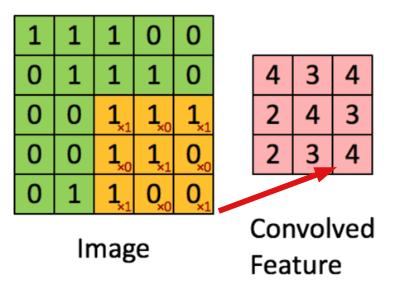
\includegraphics{img/feature_mapping.png}
\caption{feature\_mapping}
\end{figure}

\textbf{Abbildung 1}. Die Abbildung wurde aus folgendem Artikel
entnommen:
\href{https://ujjwalkarn.me/2016/08/11/intuitive-explanation-convnets/}{An
Intuitive Explanation of Convolutional Neural Networks}.

Da jeder Filter in der Eingabematrix ein bestimmtes Muster oder Konzept
erkennt, werden mehrere Filter in einem Convolutional Layer verwendet.
Je mehr Filter verwendet werden, desto mehr Features können aus den
Eingabedaten extrahiert werden (Karn, 2016). Auf jede Ausgabe eines
Convolutional Layer wird eine Aktivierungsfunktion wie z.B. die
ReLU-Funktion angewandt. Bevor die Ausgabe eines vorangegangenen
Convolution Layers an das nächste Convolution oder Dense Layer übergeben
wird, wird sie oft einem \textbf{Pooling Layer} übergeben. Die Aufgabe
eines Pooling Layers ist die Verkleinerung des Bildes mithilfe von
Pooling-Filtern, um die Anzahl der Parameter, die Rechenlast und das
Risiko von Overfitting zu verringern (Géron, 2020, S. 460). Es gibt
verschiedene Arten von Pooling, das in dieser Arbeit verwendete Pooling
ist das Max-Pooling, bei dem nur der größte Wert des Pooling Filters dem
folgenden Layer übergeben wird.

Es ist auch möglich, CNNs für andere Dateitypen zu verwenden. Da in
dieser Arbeit Textdaten verwendet werden, muss die CNN Architektur für
diese Daten angepasst werden. Anstatt zweidimensionaler Convolutional
Layer benutzt man bei Textdaten oft eindimensionale Convolutional Layer
(Géron, 2020, S. 524). Beim eindimensionalen Convolutional Layer werden
viele Filter über eine Textsequenz geschoben, womit für jeden Filter
eine eindimensionale Feature Map erzeugt wird. Somit lernt das Netz bei
jedem Filter ein einzelnes, sequenzielles Muster und die Filter können
in Kombination mit Max-Pooling relevante N-Gramme entdecken (JACOVI,
2018, S. 56). Damit können eindimensionale CNNs eine schnellere
Alternative zu Rekurrenten Neuronalen Netzen für simple Aufgaben wie die
Textklassifikation sein (CHOLLET, 2018, S. 225). Laut Goldberg sind CNNs
nützlich für Textklassikationsprobleme, bei denen es wichtige, lokale
Hinweise in den Daten hinsichtlich der Klassenzugehörigkeit gibt, die
jedoch an verschiedenen Stellen eines Dokuments auftauchen (Goldberg,
2015, S. 348). Damit eignen sich CNNs für die Entdeckung von relevanten,
positionsunabhängigen Wortfolgen, welches bei der Sentiment Analysis
z.B. aussagekräftige Wörter oder Phrasen sein können, die
Bedeutungsträger von Meinungen, Stimmungen, Einschätzungen und Emotionen
sind.

    \hypertarget{kimcnn}{%
\subsubsection{KimCNN}\label{kimcnn}}

2014 veröffentlichte Yoon Kim das Paper ``Convolutional Neural Networks
for Sentence Classification'', in welchem er eine CNN Modellarchitektur
vorstellte (Kim, 2014), welches im Verlauf dieser Arbeit ``KimCNN''
genannt wird. Zu dem Zeitpunkt konnte KimCNN in Kombination mit Word2Vec
Embeddings State-of-the-art Ergebnisse im Bereich der Textklassifikation
bei 4 von 7 getesteten Datensätzen erreichen, darunter auch bei einem
Sentiment Analysis Datensatz (Kim, 2014, S. 1746). In dieser Arbeit
wurde das Modell in Kombination mit den Word2Vec-Nachfolgern
\textbf{GloVe} und \textbf{FastText} verwendet. Zudem wurde nur die
Version ``CNN-non-static'' verwendet, bei welcher die vortrainierten
Word Embeddings für die entsprechende Aufgabe gefinetuned werden. Bei
KimCNN werden die Convolutions wortweise über die Eingabevektoren
berechnet, wobei unterschiedlich große Filterfenster (Werte: 3, 4, 5)
für die gleichzeitige Verarbeitung von Wörtern verwendet wurden. Die
resultierenden Feature-Maps wurden mit einem Max-Pooling-Layer
verarbeitet, um die extrahierten Features zu verdichten oder
zusammenzufassen. Das Modell sieht wie folgt aus:

\begin{Shaded}
\begin{Highlighting}[]
\NormalTok{KimCNN(}
\NormalTok{  (embedding): Embedding(}\DecValTok{25002}\NormalTok{, }\DecValTok{300}\NormalTok{, padding\_idx}\OperatorTok{=}\DecValTok{1}\NormalTok{)}
\NormalTok{  (convs): ModuleList(}
\NormalTok{    (}\DecValTok{0}\NormalTok{): Conv1d(}\DecValTok{1}\NormalTok{, }\DecValTok{100}\NormalTok{, kernel\_size}\OperatorTok{=}\NormalTok{(}\DecValTok{3}\NormalTok{, }\DecValTok{300}\NormalTok{), stride}\OperatorTok{=}\NormalTok{(}\DecValTok{1}\NormalTok{,))}
\NormalTok{    (}\DecValTok{1}\NormalTok{): Conv1d(}\DecValTok{1}\NormalTok{, }\DecValTok{100}\NormalTok{, kernel\_size}\OperatorTok{=}\NormalTok{(}\DecValTok{4}\NormalTok{, }\DecValTok{300}\NormalTok{), stride}\OperatorTok{=}\NormalTok{(}\DecValTok{1}\NormalTok{,))}
\NormalTok{    (}\DecValTok{2}\NormalTok{): Conv1d(}\DecValTok{1}\NormalTok{, }\DecValTok{100}\NormalTok{, kernel\_size}\OperatorTok{=}\NormalTok{(}\DecValTok{5}\NormalTok{, }\DecValTok{300}\NormalTok{), stride}\OperatorTok{=}\NormalTok{(}\DecValTok{1}\NormalTok{,))}
\NormalTok{  )}
\NormalTok{  (fc): Linear(in\_features}\OperatorTok{=}\DecValTok{300}\NormalTok{, out\_features}\OperatorTok{=}\DecValTok{3}\NormalTok{, bias}\OperatorTok{=}\VariableTok{True}\NormalTok{)}
\NormalTok{  (dropout): Dropout(p}\OperatorTok{=}\FloatTok{0.5}\NormalTok{, inplace}\OperatorTok{=}\VariableTok{False}\NormalTok{)}
\NormalTok{)}
\end{Highlighting}
\end{Shaded}

Die Werte bedeuten folgendes: - \(25002\) (embedding): Größe des
Vokabulars (= die maximale Anzahl an Features) plus ein Token für
unbekannte Wörter \texttt{\textless{}UNK\textgreater{}} und ein
Padding-Token \texttt{\textless{}PAD\textgreater{}} - \(300\)
(embedding): Dimension des Embeddings - \(100\) (convs): Anzahl der
Filter - \(3, 4, 5\) (convs): Filtergrößen - \(3\) (fc): Anzahl der
Klassen (positiv, neutral, negativ) - \(0.5\) (dropout): Dropoutrate

KimCNN verwendete folgende Parameter, die mithilfe von GridSearch für
alle von Kim getesteten Datensätze die besten Ergebnisse lieferten und
auch für die Experimente in dieser Arbeit verwendet wurden:

\begin{itemize}
\tightlist
\item
  Aktivierunsfunktion: ReLU
\item
  Filtergrößen: 3, 4, 5
\item
  Anzahl der Filter: 100
\item
  Dropoutrate: 0.5
\item
  Batchgröße: 50
\item
  Optimierungsverfahren: Adadelta
\end{itemize}

    \hypertarget{maschinelle-lernverfahren}{%
\subsection{Maschinelle Lernverfahren}\label{maschinelle-lernverfahren}}

Für die Experimente in dieser Arbeit wurden neben KimCNN und einem
\emph{fine-tuned} BERT-Modell die Machine Learning Verfahren Logistic
Regression und Support Vector Machines für die Sentiment Analysis
verwendet. Sie sind etablierte Verfahren, die schon seit Jahrzehnten zur
Textklassifikation verwendet werden (Kowsari, 2019, S. 3, 20f.). Anders
als KimCNN oder das BERT-Modell nutzten diese Verfahren in dieser Arbeit
keine vortrainierten Gewichte, sondern wurden ``from scratch''
trainiert, d.h. alle Informationen, die zur Klassifizierung verwendet
wurden, wurden lediglich aus de Trainingsdaten gewonnen. Zur
Vektorisierung der Wörter wurde anstelle von Word Embeddings ein
Bag-of-Words Modell mit einer TF-IDF-Gewichtung verwendet, bei dem die
Häufigkeit eines Wortes im Verhältnis zur Häufigkeit im gesamten Korpus
berücksichtigt und gegebenenfalls niedriger gewichtet wird. Die
Experimente mit den Machine Learning Verfahren sollten ein Gegenentwurf
zu den anderen Ansätzen darstellen, da sie auf Informationen aus
vortrainierten Embeddings verzichten und stattdessen nur die
Informationen aus dem Nutzerreview-Korpus zur Sentiment Analysis
verwenden. Weiterhin sollte überprüft werden, wie hoch die Auswirkung
der simpleren Darstellung der Wörter durch hochdimensionale,
dünnbesetzte Vektoren im Vergleich zu den weniger hochdimensionalen,
dichtbesetzten Embbeddings hinsichtlich der Klassifizierungsgenauigkeit
ausfallen würde.

    \hypertarget{experimente}{%
\section{Experimente}\label{experimente}}

\hypertarget{aufbau}{%
\subsection{Aufbau}\label{aufbau}}

Für die Experimente wurden Stoppwörter beibehalten, um die Größe der im
Durchschnitt sehr kurzen Reviews (\textasciitilde49 Tokens) nicht noch
weiter zu verringern. Alle Wörter wurden durch kleingeschriebene Wörter
dargestellt. Das Korpus wurde für die Experimente in einen Trainings-,
Validierungs- und Testdatensatz aufgeteilt. Die Aufteilung erfolgte nach
dem Pareto-Prinzip, d.h. 80\% der Daten wurden als Trainingsdaten
verwendet und jeweils 10\% für die Validierungs- und Testdaten. Dies
wurde dreimal durchgeführt, sodass eine dreifache Kreuzvalidierung
durchgeführt werden konnte. Die Genauigkeit wurde bei jeder
Kreuzvalidierung für den Testdatensatz berechnet und dann gemittelt. Für
die Messung der Genauigkeit wurde die \textbf{Categorical Accuracy}
verwendet, welche mit der folgenden Formel berechnet wird:

\(\text{Categorical Accuracy} = \dfrac{\text{Anzahl der korrekten Voraussagen}}{\text{Gesamtanzahl aller Voraussagen}}\)

    Für die unterschiedlichen Embeddings wurden eine Reihe von
vortrainierten Embeddings verwendet (siehe Tabelle 2). Für jedes
Embedding (außer den BERT Embeddings) wurde in Kombination mit KimCNN
eine Hyperparameteroptimierung durchgeführt, bei der folgende Parameter
und Werte optimiert wurden: - Batchgröße: 50, 128 - Lernrate: 0.01,
0.001 - Maximale Anzahl an Features: 25000, 50000 - Maximale Anzahl an
Epochen: 500

Die Batchgröße wurde einmal auf 50 gestellt, da dies bei den
Experimenten von Kim die besten Ergebnisse lieferte (Kim, 2014, S. 1748)
und als Vergleich auf eine größere Batchgröße von 128. Die maximale
Anzahl an Epochen wurde auf 500 gestellt, jedoch wurde Early Stopping
mit einer Patience von 3 eingebaut, sodass das Netz aufhörte zu
trainieren, sobald sich der Validierungs Loss drei Epochen lang nicht
verringerte.

\begin{longtable}[]{@{}llll@{}}
\toprule
\begin{minipage}[b]{0.03\columnwidth}\raggedright
Embedding\strut
\end{minipage} & \begin{minipage}[b]{0.07\columnwidth}\raggedright
Modell\strut
\end{minipage} & \begin{minipage}[b]{0.67\columnwidth}\raggedright
Details\strut
\end{minipage} & \begin{minipage}[b]{0.11\columnwidth}\raggedright
Link\strut
\end{minipage}\tabularnewline
\midrule
\endhead
\begin{minipage}[t]{0.03\columnwidth}\raggedright
\textbf{BERT}\strut
\end{minipage} & \begin{minipage}[t]{0.07\columnwidth}\raggedright
bert-base-uncased\strut
\end{minipage} & \begin{minipage}[t]{0.67\columnwidth}\raggedright
12-layer, 768-hidden, 12-heads, 110M parameters. Wurde auf
kleingeschriebenen englischen Texten trainiert.\strut
\end{minipage} & \begin{minipage}[t]{0.11\columnwidth}\raggedright
https://huggingface.co/transformers/pretrained\_models.html (abgerufen
am 23.08.2020).\strut
\end{minipage}\tabularnewline
\begin{minipage}[t]{0.03\columnwidth}\raggedright
\textbf{FastText}\strut
\end{minipage} & \begin{minipage}[t]{0.07\columnwidth}\raggedright
fasttext.en.300d\strut
\end{minipage} & \begin{minipage}[t]{0.67\columnwidth}\raggedright
Eine Million Wortvektoren wurden auf einem Wiki-Korpus von 2017, dem
UMBC Korpus und dem statmt.org Nachrichtenkorpus erstellt. Die Sprache
ist Englisch.\strut
\end{minipage} & \begin{minipage}[t]{0.11\columnwidth}\raggedright
https://fasttext.cc/docs/en/english-vectors.html (abgerufen am
23.08.2020).\strut
\end{minipage}\tabularnewline
\begin{minipage}[t]{0.03\columnwidth}\raggedright
\textbf{FastText}\strut
\end{minipage} & \begin{minipage}[t]{0.07\columnwidth}\raggedright
fasttext.simple.300d\strut
\end{minipage} & \begin{minipage}[t]{0.67\columnwidth}\raggedright
Eine Million Wortvektoren wurden auf einem Wiki-Korpus von 2017, dem
UMBC Korpus und dem statmt.org Nachrichtenkorpus erstellt. Die Sprache
ist einfaches Englisch.\strut
\end{minipage} & \begin{minipage}[t]{0.11\columnwidth}\raggedright
https://fasttext.cc/docs/en/english-vectors.html (abgerufen am
23.08.2020).\strut
\end{minipage}\tabularnewline
\begin{minipage}[t]{0.03\columnwidth}\raggedright
\textbf{GloVe}\strut
\end{minipage} & \begin{minipage}[t]{0.07\columnwidth}\raggedright
glove.6B.300d\strut
\end{minipage} & \begin{minipage}[t]{0.67\columnwidth}\raggedright
Diese Embeddings wurden auf einem Wiki-Korpus von 2014 und dem Gigaword
Korpus trainiert. Es beinhaltet 6 Milliarden Tokens und ein Vokabular
von 400000 Tokens.\strut
\end{minipage} & \begin{minipage}[t]{0.11\columnwidth}\raggedright
https://nlp.stanford.edu/projects/glove/ (abgerufen am 23.08.2020)\strut
\end{minipage}\tabularnewline
\begin{minipage}[t]{0.03\columnwidth}\raggedright
\textbf{GloVe}\strut
\end{minipage} & \begin{minipage}[t]{0.07\columnwidth}\raggedright
glove.840B.300d\strut
\end{minipage} & \begin{minipage}[t]{0.67\columnwidth}\raggedright
Diese Embeddings wurden auf dem Common Crawl Korpus trainiert. Es
beinhaltet 840 Milliarden Tokens und ein Vokabular von 2,2 Millionen
Tokens.\strut
\end{minipage} & \begin{minipage}[t]{0.11\columnwidth}\raggedright
https://nlp.stanford.edu/projects/glove/ (abgerufen am 23.08.2020)\strut
\end{minipage}\tabularnewline
\begin{minipage}[t]{0.03\columnwidth}\raggedright
\textbf{GloVe}\strut
\end{minipage} & \begin{minipage}[t]{0.07\columnwidth}\raggedright
glove.twitter.27B.200d\strut
\end{minipage} & \begin{minipage}[t]{0.67\columnwidth}\raggedright
Diese Embeddings wurden auf Tweets von Twitter trainiert. Es beinhaltet
2 Milliarden Tweetw, 27 Milliarden Tokens und ein Vokabular von 1,2
Millionen Tokens.\strut
\end{minipage} & \begin{minipage}[t]{0.11\columnwidth}\raggedright
https://nlp.stanford.edu/projects/glove/ (abgerufen am 23.08.2020)\strut
\end{minipage}\tabularnewline
\bottomrule
\end{longtable}

\textbf{Tabelle 2}: Auflistung aller verwendeten Embeddings.

    Für die Experimente mit dem fine-tuned BERT-Modell wurde versucht, sich
an die vorgeschlagenen Hyperparameter von Devlin et. al zu halten
(Devlin, 2018, S. 4183f.), die im Folgenden aufgelistet werden:

\begin{itemize}
\tightlist
\item
  Batchgröße: 16, 32
\item
  Lernrate: 2e-5, 3e-5, 5e-5
\item
  Anzahl der Epochen: 2, 3, 4
\item
  Optimierungsverfahren: AdamW
\item
  Maximale Anzahl an Features: 510
\end{itemize}

Die Batchgröße wurde für die Experimente in dieser Arbeit auf \(8\)
reduziert. Die Anzahl der Epochen wurde auf \(10\) erhöht und wie bei
den Experimenten mit KimCNN wurde EarlyStopping mit einer Patience von
\(2\) in das Training integriert. Die maximale Anzahl an Features ist
kleiner als bei den anderen Experimenten, da BERT standardmäßig nur eine
maximale Textlänge von 512 Tokens(FN: Tatsächlich sind es nur 510
Tokens, da noch jeweils ein Token für unbekannte Wörter und ein
Padding-Token hinzukommen.) erlaubt. Für BERT stehen mehrere
vortrainierte Modelle zur Verfügung (FN: Siehe
https://huggingface.co/transformers/pretrained\_models.html (abgerufen
am 27.08.2020).), in dieser Arbeit wurde nur das vortrainierte Modell
``bert-base-uncased'' verwendet.(FN: Es wurden auch Versuche mit
``bert-large-uncased'' gestartet, jedoch erzeugten diese sehr schlechte
Ergebnisse, da BERT Large sehr viel Ressourcen benötigt und somit nur
eine geringe Batchgröße (= \(2\)) ausgewählt werden konnte, siehe auch
https://github.com/google-research/bert\#out-of-memory-issues (abgerufen
am 27.08.2020).)

Für die Experimente mit den Machine Learning Verfahren wurde für die
Evaluation und die Hyperparameteroptimierung eine verschachtelte
Kreuzvalidierung (FN: Dabei wählt die ``innere'' Kreuzvalidierung auf
Basis der zu untersuchenden Hyperparameter das beste Modell aus und die
``äußere'' Kreuzvalidierung misst die Performance des jeweils besten
Modells.) durchgeführt, indem die zu optimierenden Hyperparameter, die
Suchräume sowie eine Pipeline mit der TF-IDF-Vektorisierung und dem
jeweiligen Klassifizierungsverfahren der Kreuzvalidierung übergeben
wurde. Durch die verschachtelte Kreuzvalidierung sollte eine möglichst
unverfälschte Bewertung der Machine Learning Verfahren gewährleistet
werden. Es wurden folgene Parameter in den Suchräumen optimiert:

\begin{itemize}
\tightlist
\item
  N-Gramme: (1,1), (1,2), (2,3)
\item
  Maximale Anzahl an Features: 25000, 50000
\item
  Toleranz: 0.01, 0.001
\item
  C: 1, 2, 3
\item
  Maximale Anzahl an Iterationen: 1000, 3000, 5000
\end{itemize}

    \hypertarget{ergebnisse}{%
\subsection{Ergebnisse}\label{ergebnisse}}

TODO: ausfüllen

\begin{longtable}[]{@{}lll@{}}
\toprule
\begin{minipage}[b]{0.14\columnwidth}\raggedright
Modell (+ Embedding)\strut
\end{minipage} & \begin{minipage}[b]{0.07\columnwidth}\raggedright
Genauigkeit\strut
\end{minipage} & \begin{minipage}[b]{0.70\columnwidth}\raggedright
Beste Parameter\strut
\end{minipage}\tabularnewline
\midrule
\endhead
\begin{minipage}[t]{0.14\columnwidth}\raggedright
BERT + bert-base-uncased\strut
\end{minipage} & \begin{minipage}[t]{0.07\columnwidth}\raggedright
76,4\strut
\end{minipage} & \begin{minipage}[t]{0.70\columnwidth}\raggedright
Batchgröße: 8Lernrate: 2e-05Maximale Anzahl an Features: 510\strut
\end{minipage}\tabularnewline
\begin{minipage}[t]{0.14\columnwidth}\raggedright
KimCNN + fasttext.en.300d\strut
\end{minipage} & \begin{minipage}[t]{0.07\columnwidth}\raggedright
71,52\strut
\end{minipage} & \begin{minipage}[t]{0.70\columnwidth}\raggedright
Batchgröße: 128Lernrate: 0.01Maximale Anzahl an Features: 50000\strut
\end{minipage}\tabularnewline
\begin{minipage}[t]{0.14\columnwidth}\raggedright
KimCNN + fasttext.simple.300d\strut
\end{minipage} & \begin{minipage}[t]{0.07\columnwidth}\raggedright
71,29\strut
\end{minipage} & \begin{minipage}[t]{0.70\columnwidth}\raggedright
Batchgröße: 128Lernrate: 0.01Maximale Anzahl an Features: 25000\strut
\end{minipage}\tabularnewline
\begin{minipage}[t]{0.14\columnwidth}\raggedright
KimCNN + glove.6B.300d\strut
\end{minipage} & \begin{minipage}[t]{0.07\columnwidth}\raggedright
TODO\strut
\end{minipage} & \begin{minipage}[t]{0.70\columnwidth}\raggedright
Batchgröße: 50, 128Lernrate: 0.01, 0.001Maximale Anzahl an Features:
25000, 50000\strut
\end{minipage}\tabularnewline
\begin{minipage}[t]{0.14\columnwidth}\raggedright
KimCNN + glove.840B.300d\strut
\end{minipage} & \begin{minipage}[t]{0.07\columnwidth}\raggedright
TODO\strut
\end{minipage} & \begin{minipage}[t]{0.70\columnwidth}\raggedright
Batchgröße: 50, 128Lernrate: 0.01, 0.001Maximale Anzahl an Features:
25000, 50000\strut
\end{minipage}\tabularnewline
\begin{minipage}[t]{0.14\columnwidth}\raggedright
KimCNN + glove.twitter.27B.200d\strut
\end{minipage} & \begin{minipage}[t]{0.07\columnwidth}\raggedright
TODO\strut
\end{minipage} & \begin{minipage}[t]{0.70\columnwidth}\raggedright
Batchgröße: 50, 128Lernrate: 0.01, 0.001Maximale Anzahl an Features:
25000, 50000\strut
\end{minipage}\tabularnewline
\begin{minipage}[t]{0.14\columnwidth}\raggedright
Logistic Regression\strut
\end{minipage} & \begin{minipage}[t]{0.07\columnwidth}\raggedright
72,4\strut
\end{minipage} & \begin{minipage}[t]{0.70\columnwidth}\raggedright
-\strut
\end{minipage}\tabularnewline
\begin{minipage}[t]{0.14\columnwidth}\raggedright
Support Vector Machines\strut
\end{minipage} & \begin{minipage}[t]{0.07\columnwidth}\raggedright
71\strut
\end{minipage} & \begin{minipage}[t]{0.70\columnwidth}\raggedright
-\strut
\end{minipage}\tabularnewline
\bottomrule
\end{longtable}

\textbf{Tabelle 3}: Die Tabelle stellt in jeder Zeile die
durschnittlichen Genauigkeiten des jeweils besten Modells sowie die
besten Parameter dar. Aufgrund der verschachtelten Kreuzvalidierung
konnten die besten Hyperparameter für die maschinellen Lernverfahren
Logistic Regression und Support Vector Machines nicht ermittelt werden.

    In Tabelle 3 werden alle verwendeten Verfahren und die
Klassifizierungsgenauigkeiten des jeweiligen Verfahrens mit den besten
Hyperparametern sowie die besten Hyperparameter dargestellt.

TODO: - Tabelle - interpretieren - bei fasttext: - keine großen
unterschiede bei max features und batch size - insgesamt sehr stabile
und gleichbleibende ergebnisse (+/- 2\% acc) - learning rate ist eig
immer 0.01 besser - bei glove: - bei bert - die ml verfahren sind
genauso gut wie kimcnns mit embeddings

TODO: hier confusion matrices - bestes cnn noch ausführlicher optimieren
- ausgewählte confusion matrix von bestem cnn und bestem bert hier
zeigen - Bei BERT sind die stärksten Fehlklassifizierungen bei Neutral
und Negativ. TODO: cnn auch? - unterschiede angucken

TODO: Besonderheiten beim Nutzerreview-Korpus sind die Kürze der Texte
und die fehlerhafte Orthographie.

Neben der reinen Klassifizierungsgenauigkeit sollten noch die Dauer des
Trainingsm, die Dauer der Hyperparameteroptimierung und die benötigte
Rechenleistung untersucht werden. Dabei sind die gemessenen Zeitwerte
nur ungefähre Richtwerte, da eine genaue Messung der Trainings- und
Optimierungsdauer viele Faktoren wie die Auslastung oder die eingebauten
Hardwarekomponenten des Computers berücksichtigen muss. Die schnellsten
Verfahren inklusive Hyperparameteroptimierung waren die Machine Learning
Verfahren, die im Schnitt für das Training mit Hyperparameteroptimierung
etwa 20 Minuten brauchten. Als einzige Verfahren konnten diese nur auf
der CPU trainiert werden, für KimCNN und BERT war zusätzlich eine GPU
nötig, um das Training zu beschleunigen. Trotzdem brauchte KimCNN für
jedes Trainings eines Embeddingmodells inklusive
Hyperparameteriptimierung etwa 15-20 Stunden. BERT benötigte etwa genau
so lange wie KimCNN, jedoch wurden auch weitaus weniger Hyperparameter
optimiert. Ist die Trainings- und Optimierungsdauer also ein wichtiger
Faktor, so sind die Machine Learning Verfahren effizienter als KimCNN,
da sie nicht nur schneller waren, sondern auch gleiche
Klassifizierungsgenauigkeiten erreichen konnten und keine GPU
benötigten. BERT benötigt ebenfalls eine GPU und erlaubt aufgrund seiner
Komplexität nur geringe Batchgrößen, konnte jedoch höhere
Klassifizierungsgenauigkeiten als die Machine Learning Verfahren oder
die KimCNNs erreichen (TODO: stimmt das?), auch wenn diese nicht
bedeutend höher ausfielen (+ \textasciitilde4\% TODO).

    \hypertarget{schlussbetrachtung}{%
\section{Schlussbetrachtung}\label{schlussbetrachtung}}

In dieser Arbeit wurde eine Sentiment Analysis anhand eines
Amazon-Nutzerreview Korpus in der Produktkategorie ``Elektronik''
durchgeführt, wobei die Sentiment Analysis als Textklassifikation
aufgefasst wurde. Für die Sentiment Analysis wurden verschiedene
Klassifizierungstechniken verwendet und miteinander verglichen. Jede
dieser Klassifizierungstechniken unterschied sich von den anderen
Techniken. Die Machine Learning Verfahren verwendeten anders als die
anderen Verfahren keine vortrainierten Wordvektoren, sondern erhielten
alle zur Klassifizierung benötigten Informationen lediglich aus den
Trainingsdaten. KimCNN ist eine simple Variante eines Convolutional
Neural Networks für Textdaten und konnte 2014 für einige
Textklassifikationsaufgaben State-of-the-art Ergebnisse erzielen. Anders
als bei den Machine Learning Verfahren wurden hier eine Reihe
verschiedener vortrainierter Embeddingmodelle der Embeddingverfahren
GloVe und FastText für die Sentiment Analysis verwendet. Die Idee war,
dass die Word Embeddings durch ihre Berücksichtigung des Wortkontextes
zu einer Verbesserung der Klassifizierungsgenauigkeit beitrugen, da so
Schlüsselwörter oder -phrasen besser erkannt und zugeordnet werden
konnten. Die letzte verwendete Klassifizierungstechnik war ein
\emph{fine-tuned} BERT-Modell. BERT ist seit zwei Jahren sehr populär,
da es bei seiner Veröffentlichung 2018 eine Reihe von State-of-the-art
Ergebnisse im Bereich des Natural Language Processing erreichen konnte.
Auch BERT benutzt Word Embeddings, jedoch sind diese Embeddings in der
Lage, dynamisch den Kontext eines Wortes zu repräsentieren und somit
Worte mit gleicher Schreibweise aber unterschiedlicher Bedeutung
voneinander zu unterscheiden.

TODO: die Ergebnisse nennen

    \hypertarget{literaturverzeichnis}{%
\section{Literaturverzeichnis}\label{literaturverzeichnis}}

BOJANOWSKI, Piotr, GRAVE, Edouard, JOULIN, Armand, MIKOLOV, Tomas,
``Enriching Word Vectors with Subword Information'', in: Transactions of
the Association for Computational Linguistics, Bd. 5, Juli 2016, S.
135-146.

CHOLLET, Francois, Deep learning with Python, 2018.

DEVLIN, Jacob, CHANG, Ming-Wei, LEE, Kenton, TOUTANOVA, Kristin, ``BERT:
Pre-training of Deep Bidirectional Transformers for Language
Understanding'', in: Proceedings of the NAACL-HLT Conference, S.
4171--4186.

GéRON, Aurélien, Praxiseinstieg Machine Learning mit Scikit-Learn, Keras
und TensorFlow, übers. v. Kristian Rother und Thomas Demmig,
\({^2}2020\).

GOLDBERG, Yoav, A Primer on Neural Network Models for Natural Language
Processing, in: Journal Of Artificial Intelligence Research, Bd. 57
(2016), S. 345-420.

KARN, Ujjwal, An Intuitive Explanation of Convolutional Neural Networks,
https://ujjwalkarn.me/2016/08/11/intuitive-explanation-convnets/
(abgerufen am 20.08.2020).

KIM, Yoon, Convolutional Neural Networks for Sentence Classification,
in: Proceedings of the 2014 Conference on Empirical Methods in Natural
Language Processing (Oktober 2014), S. 1746-1751.

KOWSARI, Kamran et . al., Text Classification Algorithms. A Survey,
ArXiv 2019, S. 1-68.

JACOVI, Alon, SHALOM, Oren Sar, GOLDBERG, Yoav, Understanding
Convolutional Neural Networks for Text Classification, in: Proceedings
of the 2018 EMNLP Workshop BlackboxNLP. Analyzing and Interpreting
Neural Networks for NLP (Januar 2018), S. 56-65.

LIU, Bing, Sentiment analysis. Mining opinions, sentiments, and
emotions, Cambridge 2015.

PENNIGTON, Jeffrey, SOCHER, Richard, MANNING, Christopher D., ``GloVe:
Global Vectors for Word Representation'', in: EMNLP (Januar 2014), S.
1532-1533.

PETROLITO, Ruggero, DELL'ORLETTA, Felice, Word Embeddings in Sentiment
Analysis, in: Proceedings of the Fifth Italian Conference on
Computational Linguistics CLiC-it (Januar 2018), S. 330-334.

PILEHVAR, Mohammad Taher, CAMACHO-COLLADOS, Jose, ``Embeddings in
Natural Language Processing. Theory and Advances in Vector
Representation of Meaning'', 2020.

WEIDMAN, Seth, Deep Learning. Grundlagen und Implementierung, übers. v.
Jorgen W. Lang, 2020.

    \hypertarget{appendix}{%
\section{Appendix}\label{appendix}}

\hypertarget{daten-und-code}{%
\subsection{Daten und Code}\label{daten-und-code}}

Alle Daten und alle zur Klassifizierung verwendeten Skripte befinden
sich im Github-Repository \texttt{wordembeddings}.(FN: Siehe
https://github.com/realjanpaulus/wordembeddings.) In der folgenden
Auflistung werden die Ordner und ihre Inhalte kurz erläutert:

\begin{itemize}
\tightlist
\item
  \textbf{app}. In diesem Ordner befinden sich die zur Klassifizierung
  und Optimierung verwendeten Skripte \texttt{cnn.py}, \texttt{bert.py},
  \texttt{ml.py}, \texttt{run.py}, \texttt{run\_bert.py} sowie das
  Helferskript \texttt{utils.py} und die Datei \texttt{models.py},
  welche die KimCNN Architektur beinhaltet. Das Notebook
  \texttt{processing\_and\_results.ipynb} wurde für die Vorverarbeitung
  des Korpus und zur Zusammenfassung der Klassifizierungsergebnisse
  genutzt.
\item
  \textbf{corpora}. In diesem Ordner befindet sich das
  Amazon-Nutzerreview-Korpus und die für die Kreuzvalidierung
  verwendeten Teilkorpora.
\item
  \textbf{results}. In diesem Ordner befinden sich die Ergebnisse der
  Klassifizierungsexperimente als Textdateien sowie Grafiken der
  Konfusionsmatrizen und des Trainings- und Validierungs-Loss der CNNs
  und des BERT-Modells.
\end{itemize}

    \begin{tcolorbox}[breakable, size=fbox, boxrule=1pt, pad at break*=1mm,colback=cellbackground, colframe=cellborder]
\prompt{In}{incolor}{ }{\boxspacing}
\begin{Verbatim}[commandchars=\\\{\}]

\end{Verbatim}
\end{tcolorbox}


    % Add a bibliography block to the postdoc
    
    
    
\end{document}
